\section{Timeline Simulation and Scenario Selection}
\label{chap:dataDescription}

\todo{just to remember the red line: How are the different time series generated?}
To develop robust and generally applicable bidding strategies, high-quality data is essential.
Inaccurate or poorly constructed datasets inevitably lead to misleading results and suboptimal strategies.

There are various approaches to generating such time series data.
We begin with an overview of real-world market data in order to better understand
the patterns we aim to replicate or predict, and to identify the key characteristics
of the respective electricity markets.

To that end, the market data is first analyzed and visualized using descriptive statistics.
Subsequently, different analytical methods are discussed, combined, and applied.
This section provides a detailed examination of various techniques for generating representative time series for the  various markets.

The data used in this Chapter is from the ENTSOE transparency platform \cite{.08.04.2025} \& Regelleistung.net \cite{50HertzTransmissionGmbHAmprionGmbHTenneTTSOGmbH.18.04.2025}.

\subsection{aFFR - Capacity}

In the first panel of the overview [\ref{fig:Overview Average Negativ Capacity Price}],
the real market data from 2023 for the negative capacity market price is displayed.
Below that, the corresponding trend and seasonality components are illustrated.

\begin{figure}[!h]
	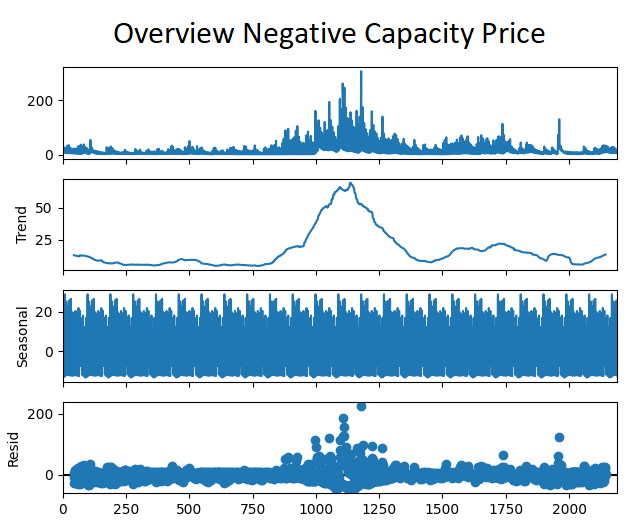
\includegraphics[width=0.7\linewidth]{pictures/capacityData_overview.png}
	\caption{Total Average Negative Capacity Price}
	\label{fig:Overview Average Negativ Capacity Price}
\end{figure}

A more detailed examination of the seasonality reveals both a daily
and a slight weekly rhythm in the data. Since the dataset refers to 4-hour blocks, every six time lags
correspond to a full day. Figure~\ref{fig:Autocorrelation Negative Capacity Price - 5 Days}
clearly illustrates the presence of a daily pattern in the autocorrelation of the data.

\begin{figure}[!h]
	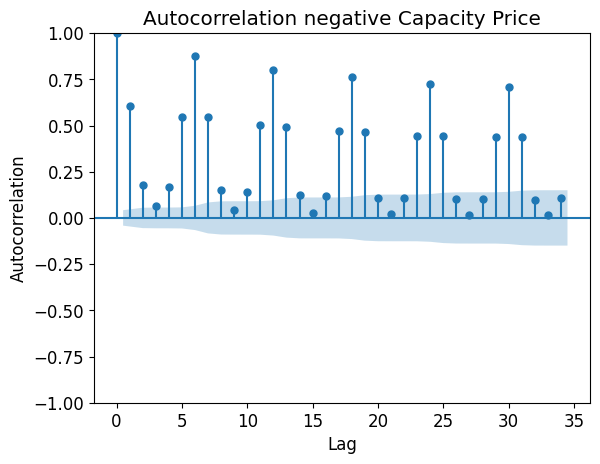
\includegraphics[width=0.7\linewidth]{pictures/Autocorrelation negative Capacity Price.png}
	\caption{Autocorrelation Negative Capacity Price – 5 Days}
	\label{fig:Autocorrelation Negative Capacity Price - 5 Days}
\end{figure}

Moreover, Figure \ref{fig:AutocorrNegCap4Weeks} indicates a moderate weekly cycle.

\begin{figure}[!h]
	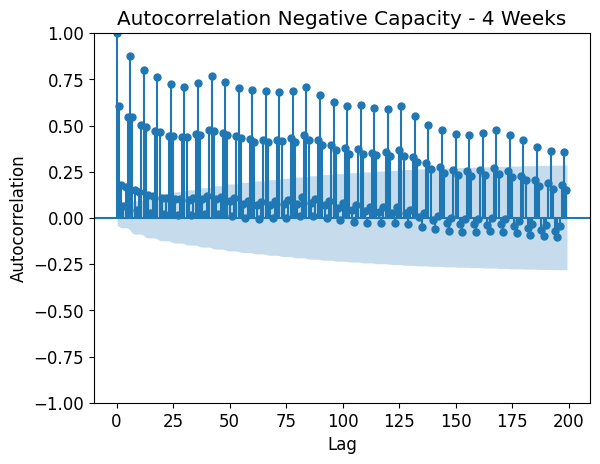
\includegraphics[width=0.7\linewidth]{pictures/Autocorrelation Negative Capacity - 4 Weeks.png}
	\caption{Autocorrelation Negative Capacity Price – 4 Weeks}
	\label{fig:AutocorrNegCap4Weeks}
\end{figure}

The price development for positive capacity shows a similar behavior
to that of the negative capacity prices.

Given the strong autocorrelation in the data, several statistical methods are well-suited
for time series analysis and forecasting. In particular, the ARIMA method,
which is based on autoregression, proves to be effective for time series
with strong autocorrelation. To better account for seasonal effects,
a seasonal variant of the ARIMA method SARIMA can be applied.
But SARIMA struggles with complexity in long time series:
computation times increased exponentially, and long-term forecasts tended to be biased
towards the most recent trend.
Since we expect similar annual patterns in the short term, this bias toward the latest trend
is considered unrealistic and undesirable.
Moreover, SARIMA is inherently limited to modeling a single seasonal component.
To account for multiple seasonalities, extensive manual adjustments would be necessary.

A more flexible alternative is the TBATS algorithm, which builds upon similar principles
while overcoming these limitations. TBATS stands for Trigonometric seasonality,
Box-Cox transformation, ARMA errors, Trend, and Seasonal components.
It is implemented in the SKTIME framework and enables efficient forecasting
of time series with multiple seasonal patterns~\cite{.05.04.2025}.

The resulting forecasted time series closely resembles the actual historical time series
(Figure~\ref{fig:Negative Capacity Price Prediction - 2023}).
Note that the time series shown here corresponds to the most probable scenario—
meaning that 50\% of all possible forecast values lie above, and 50\% lie below the prediction.

When generating longterm forecast scenarios using the trained predictor,
the inherent uncertainty increases with forecasting horizon,
resulting in a wider prediction interval
(Figure~\ref{fig:Negative Capacity Price Prediction Interval - 2023}).
While this is methodologically sound and suitable for many use cases,
we assume that the mean forecast does not lose accuracy over time
and use it as the basis for scenario generation.

\begin{figure}[!h]
	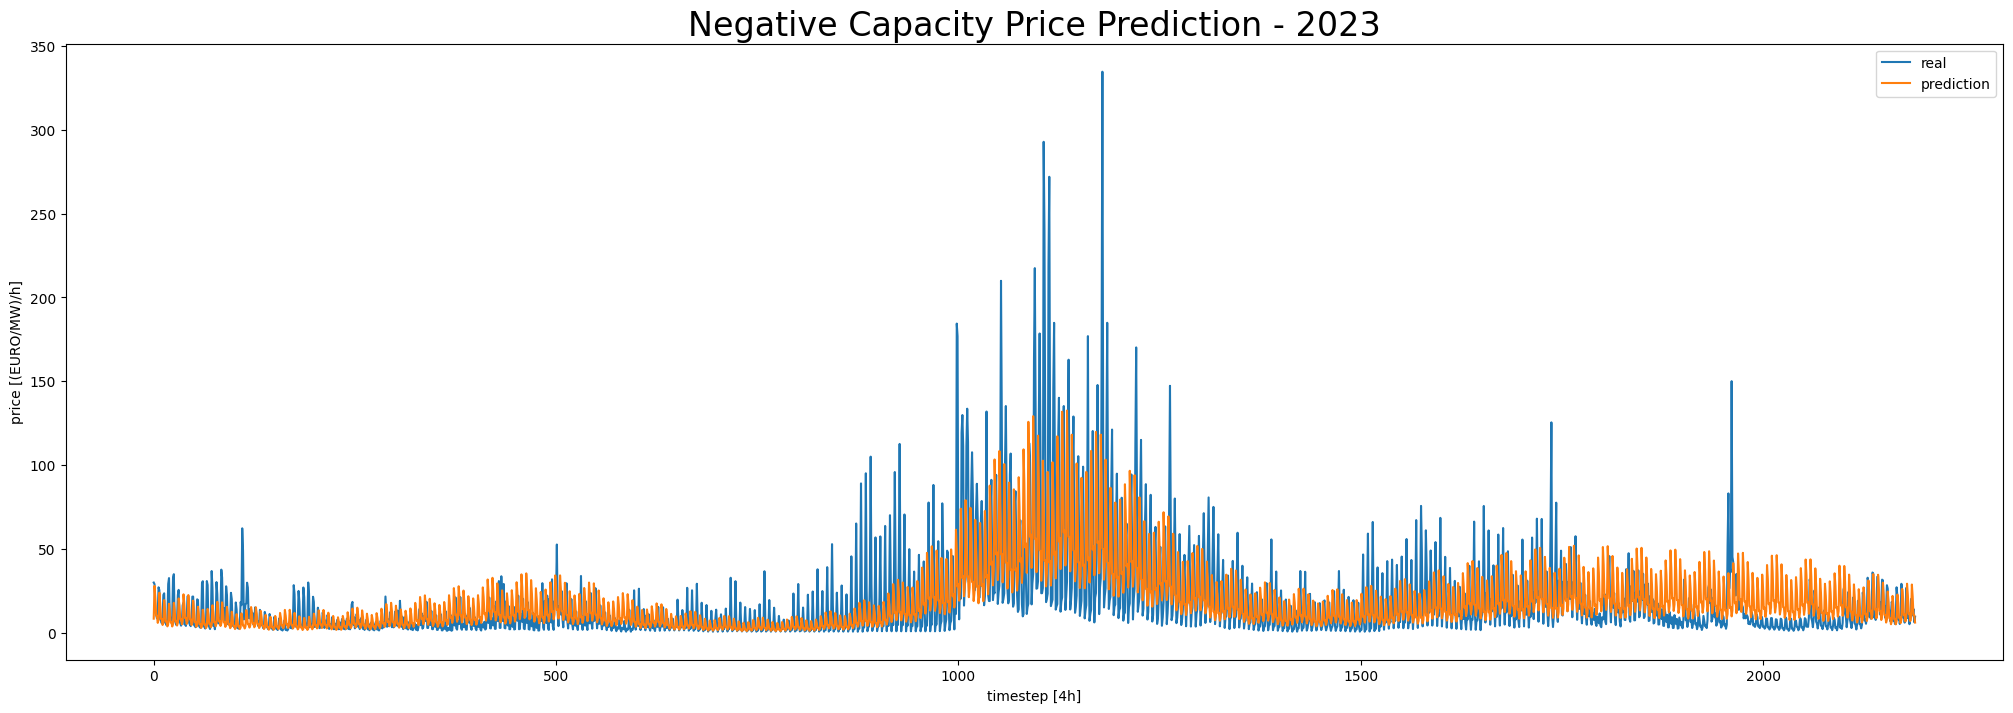
\includegraphics[width=1\linewidth]{pictures/RL/Negative Capacity Price Prediction - 2023.png}
	\caption{Negative Capacity Price Prediction – 2023}
	\label{fig:Negative Capacity Price Prediction - 2023}
\end{figure}

\begin{figure}[H]
	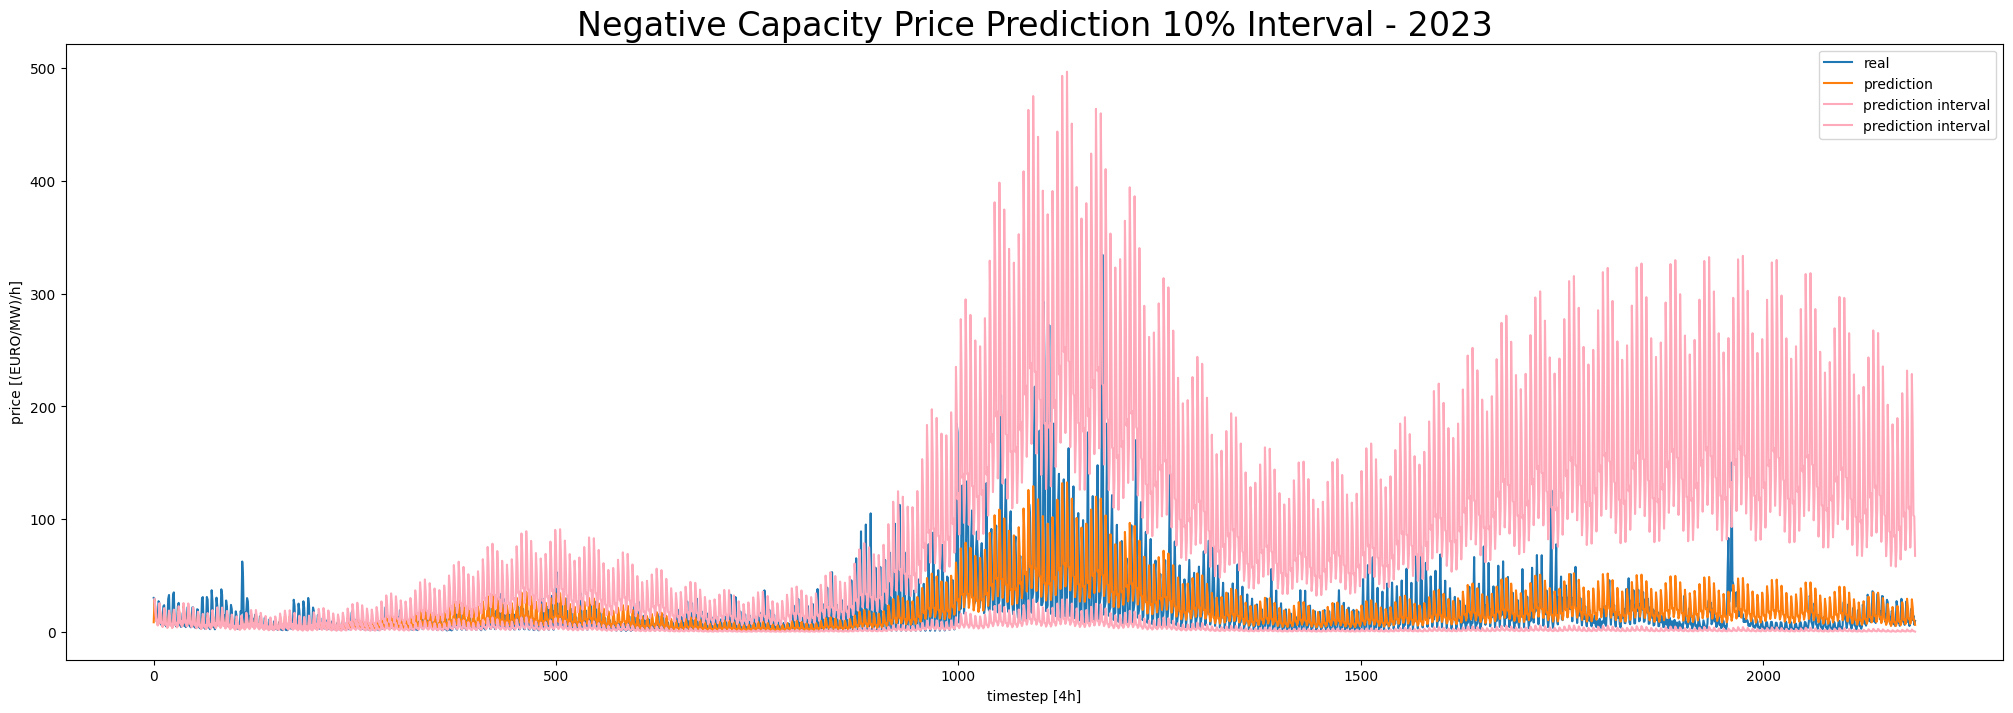
\includegraphics[width=1\linewidth]{pictures/RL/Negative Capacity Price Prediction Interval - 2023.png}
	\caption{Negative Capacity Price Prediction 10\%-Interval – 2023}
	\label{fig:Negative Capacity Price Prediction Interval - 2023}
\end{figure}

For scenario generation, the median forecast is used and manually scaled upward and downward (e.g., by ±10\%).
These scaled series are then evaluated to determine in how many cases a bidding success would have occurred.


\subsection{Day Ahead Market}

Although the Day-Ahead market prices are variable, they exhibit a daily and weekly rhythm.
Over the course of the year, only general trends are observable, as shown in Figure~\ref{fig:overviewDAprices}.

\begin{figure}[!h]
	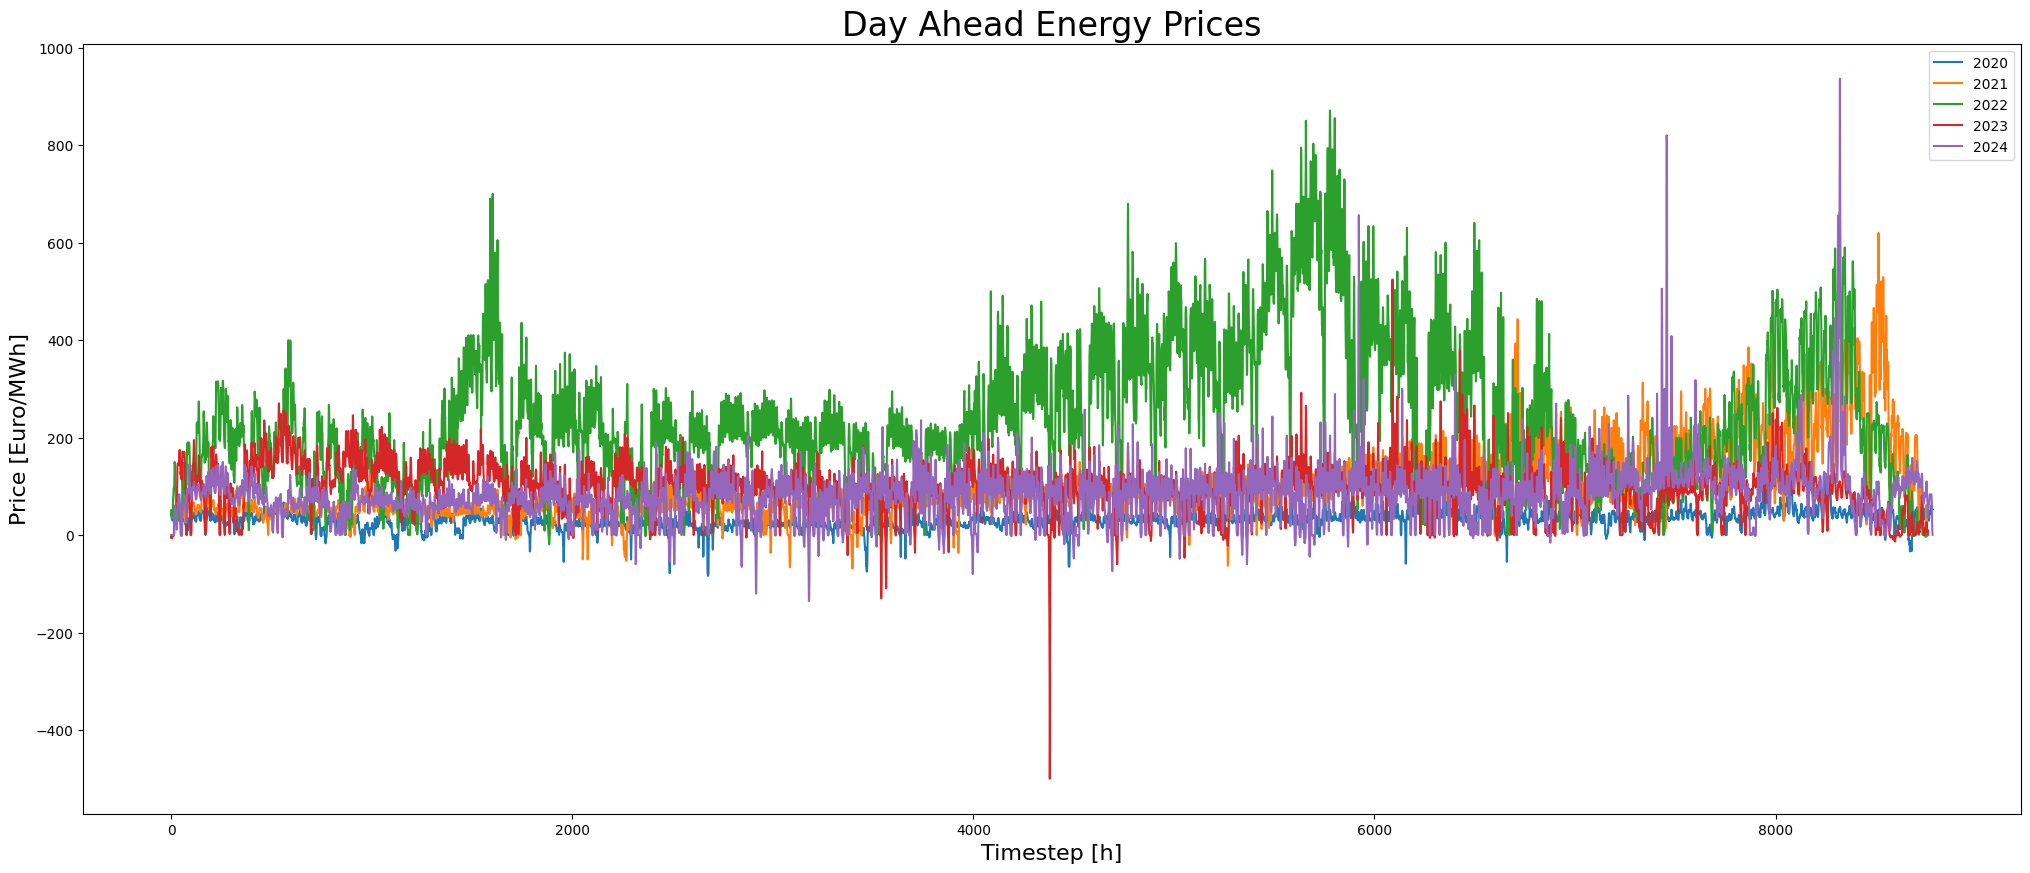
\includegraphics[width=1\linewidth]{pictures/overviewDAprices_year.png}
	\caption{Overview DA prices}
	\label{fig:overviewDAprices}
\end{figure}
\todo{redo figure with bigger legend}

The extraordinary curve movement observed in 2022 (green curve) can be attributed to
Russia's war of aggression against Ukraine and the resulting turmoil
in the gas market.

Since the Day-Ahead (DA) market operates on a pay-as-cleared mechanism
(i.e., all participants receive the price of the highest accepted bid),
and we act as a producer of renewable energy with very low operational costs,
the model only needs to consider whether we participate in the market
and what the expected clearing price is.

As illustrated in Figures \ref{fig:meanDA2020} to \ref{fig:stdDA2024},
the clearing price exhibits both daily and weekly periodicities.
While the overall level of prices may vary, the pattern remains predictable.
Due to the market design, it is sufficient for our model to rely
on an expected clearing price, as we can realistically submit
a zero-price bid and are therefore almost guaranteed to be dispatched.

The expected price used in our model is calculated as the average
of the years 2020 through 2024, excluding 2022. This approach
preserves the seasonal structure of the data while smoothing out
extreme outliers in both directions. Consequently, a reliably
expected clearing price can be determined based on time of day,
day of the week, and time of year.

Furthermore, the price level can be adjusted afterward using
a simple scaling factor without compromising the inherent
structure of the data.


\begin{figure}[H]
	\centering
	\begin{minipage}{0.49\textwidth}
		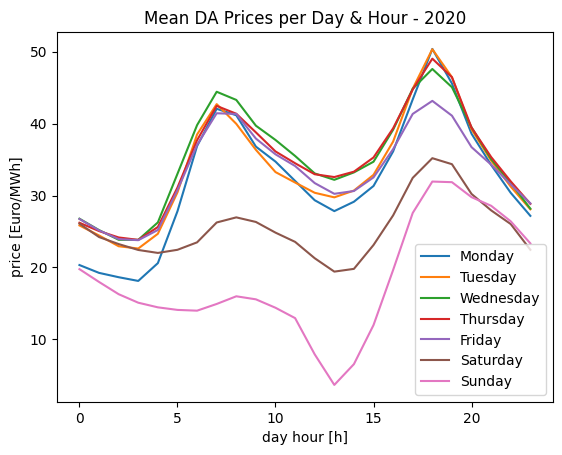
\includegraphics[width=1\linewidth]{pictures/DA/Mean DA Prices per Day and Hour - 2020.png}
		\subcaption{Mean DA-Price}
		\label{fig:meanDA2020}
	\end{minipage} \hfill
	\begin{minipage}{0.49\textwidth}
		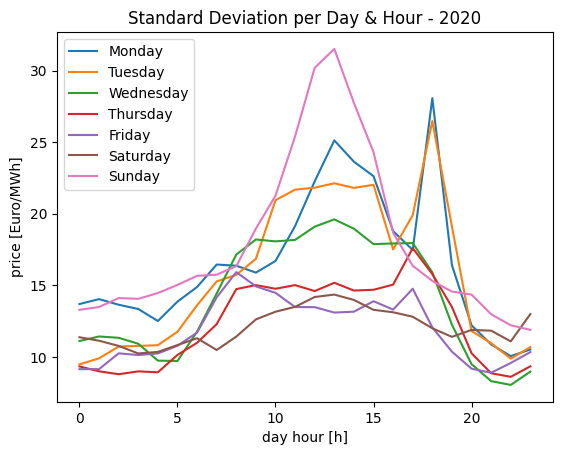
\includegraphics[width=1\linewidth]{pictures/DA/Standard Deviation per Day and Hour - 2020.png}
		\subcaption{Standard Deviation DA-Price}
		\label{fig:stdDA2020}
	\end{minipage}
	\caption{Daily and hourly DA-Data - 2020 }
\end{figure}

\begin{figure}[H]
	\centering
	\begin{minipage}{0.49\textwidth}
		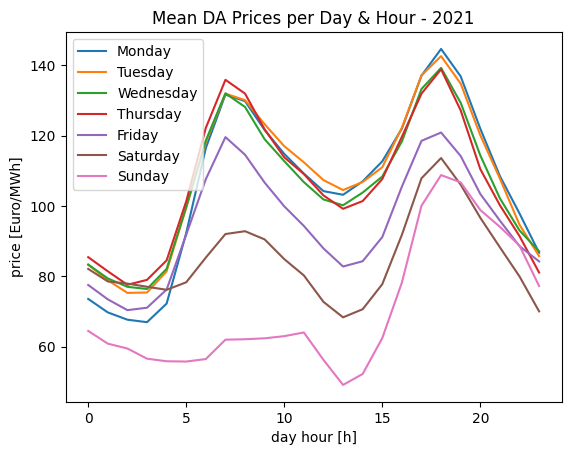
\includegraphics[width=1\linewidth]{pictures/DA/Mean DA Prices per Day and Hour - 2021.png}
		\subcaption{Mean DA-Price }
		\label{fig:meanDA2021}
	\end{minipage} \hfill
	\begin{minipage}{0.49\textwidth}
		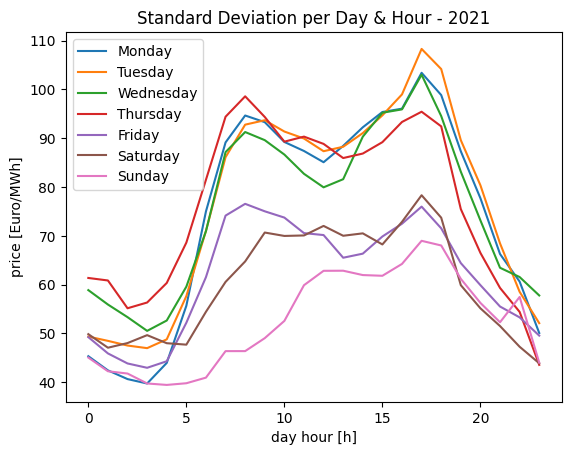
\includegraphics[width=1\linewidth]{pictures/DA/Standard Deviation per Day and Hour - 2021.png}
		\subcaption{Standard Deviation DA-Price}
		\label{fig:stdDA2021}
	\end{minipage}
	\caption{Daily and hourly DA-Data - 2021 }
\end{figure}

\begin{figure}[H]
	\centering
	\begin{minipage}{0.49\textwidth}
		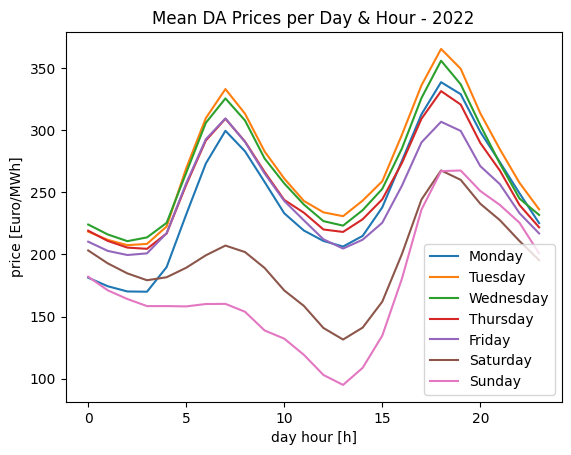
\includegraphics[width=1\linewidth]{pictures/DA/Mean DA Prices per Day and Hour - 2022.png}
		\subcaption{Mean DA-Price }
		\label{fig:meanDA2022}
	\end{minipage} \hfill
	\begin{minipage}{0.49\textwidth}
		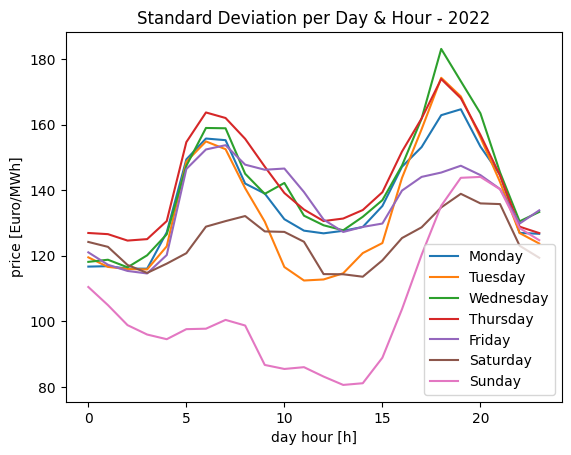
\includegraphics[width=1\linewidth]{pictures/DA/Standard Deviation per Day and Hour - 2022.png}
		\subcaption{Standard Deviation DA-Price}
		\label{fig:stdDA2022}
	\end{minipage}
	\caption{Daily and hourly DA-Data - 2022 }
\end{figure}

\begin{figure}[H]
	\centering
	\begin{minipage}{0.49\textwidth}
		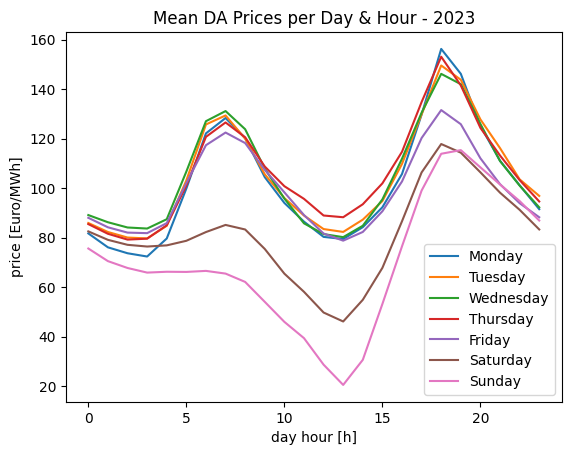
\includegraphics[width=1\linewidth]{pictures/DA/Mean DA Prices per Day and Hour - 2023.png}
		\subcaption{Mean DA-Price }
		\label{fig:meanDA2023}
	\end{minipage} \hfill
	\begin{minipage}{0.49\textwidth}
		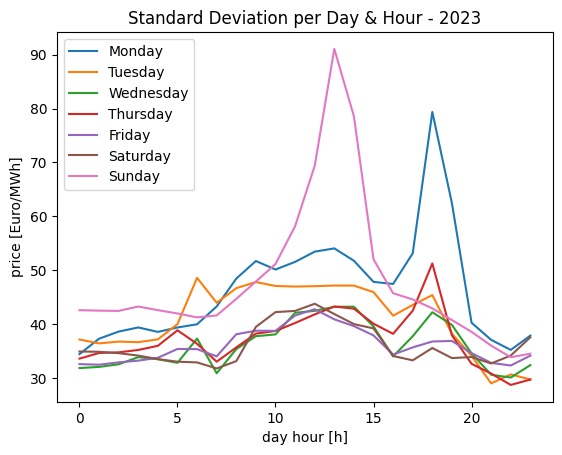
\includegraphics[width=1\linewidth]{pictures/DA/Standard Deviation per Day and Hour - 2023.png}
		\subcaption{Standard Deviation DA-Price}
		\label{fig:stdDA2023}
	\end{minipage}
	\caption{Daily and hourly DA-Data - 2023 }
\end{figure}

\begin{figure}[H]
	\centering
	\begin{minipage}{0.49\textwidth}
		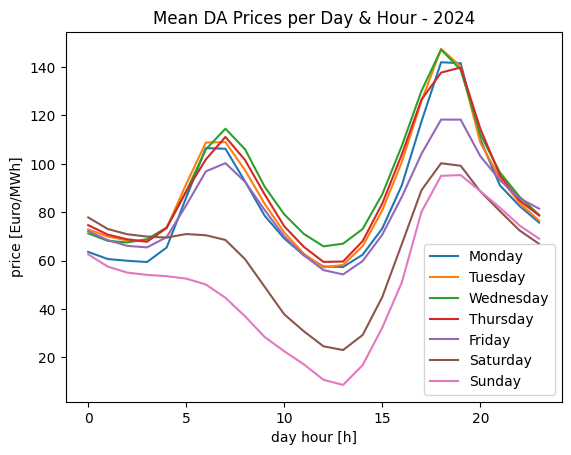
\includegraphics[width=1\linewidth]{pictures/DA/Mean DA Prices per Day and Hour - 2024.png}
		\subcaption{Mean DA-Price }
		\label{fig:meanDA2024}
	\end{minipage} \hfill
	\begin{minipage}{0.49\textwidth}
		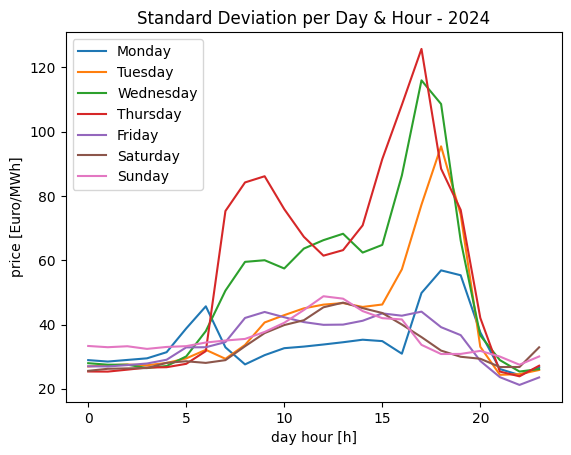
\includegraphics[width=1\linewidth]{pictures/DA/Standard Deviation per Day and Hour - 2024.png}
		\subcaption{Standard Deviation DA-Price}
		\label{fig:stdDA2024}
	\end{minipage}
	\caption{Daily and hourly DA-Data - 2024 }
\end{figure}

Additionally, for the purpose of our simulation, we assume that the
simulated renewable energy system represents an onshore wind farm
located in Germany. To obtain a wind profile, we divide the total
onshore wind power generation by the total installed capacity
of these systems \cite{.08.04.2025}.

The resulting profile reflects the mean relative wind power output over the entire
country. Because wind turbines across Germany are rarely
operating simultaneously at zero or full capacity, there are no peaks in this view.
In contrast, for an individual wind park, full or zero output can indeed occur. Therefore, in order to give
the constraint on maximum grid connection capacity a meaningful interpretation,
this average profile needs to be rescaled.

To this end, we treat the national wind production as a proxy for
the wind conditions at our specific location. We then apply a scaling
transformation that compresses the lower values and expands the higher ones.
An additional requirement of the transformation is that the maximum values
should be normalized to 1, which corresponds to our wind park operating
at full capacity.

This is achieved by first subtracting the mean of the national wind
profile, resulting in a series of positive and negative deviations.
We then apply a scaling factor to amplify these deviations both
upward and downward. Afterward, we add back the original mean to preserve
the average and total energy content of the original profile.
This transformation yields a new time series whose average matches
the original, but whose minimum is 0 and maximum value reaches 1 [\ref{eq:windProfil_our}].


\begin{flalign}
	wp_{our} = ((wp_{ger} - \bar{wp_{ger}}) * wsf) + \bar{wp_{ger}} \label{eq:windProfil_our}
\end{flalign}

The scaling factor is calculated as follows:

\begin{flalign}
	wsf = \frac{1-\bar{wp_{ger}}}{\max(wp_{ger}) - \bar{wp_{ger}}} \label{eq:windProfil_wsf}
\end{flalign}


\subsection{aFFR - Energy}
\label{chap:affR_energy}

The aFFR energy market exhibit a high degree of variability and are extremely difficult to predict statistically.
As such, they exhibit only a very weak autocorrelation, with only a slight daily rhythm, as shown in Figure
\ref{fig:Autocorrelation Positive Energy Price} (1 lag = 15 min).

\begin{figure}[!h]
	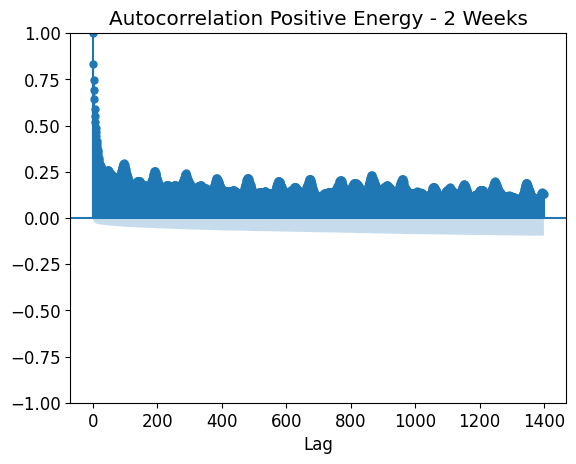
\includegraphics[width=1\linewidth]{pictures/Autocorrelation Positive Energy - 2 Weeks.png}
	\caption{Total Average Positive Energy Price}
	\label{fig:Autocorrelation Positive Energy Price}
\end{figure}

No trends are present in the data either.
As shown in Figure \ref{fig:posEngOverview}, we present 30-day samples from the early, middle, and late parts of the year.
In these periods, neither trends nor seasonal developments are observable.

\begin{figure}[!h]
	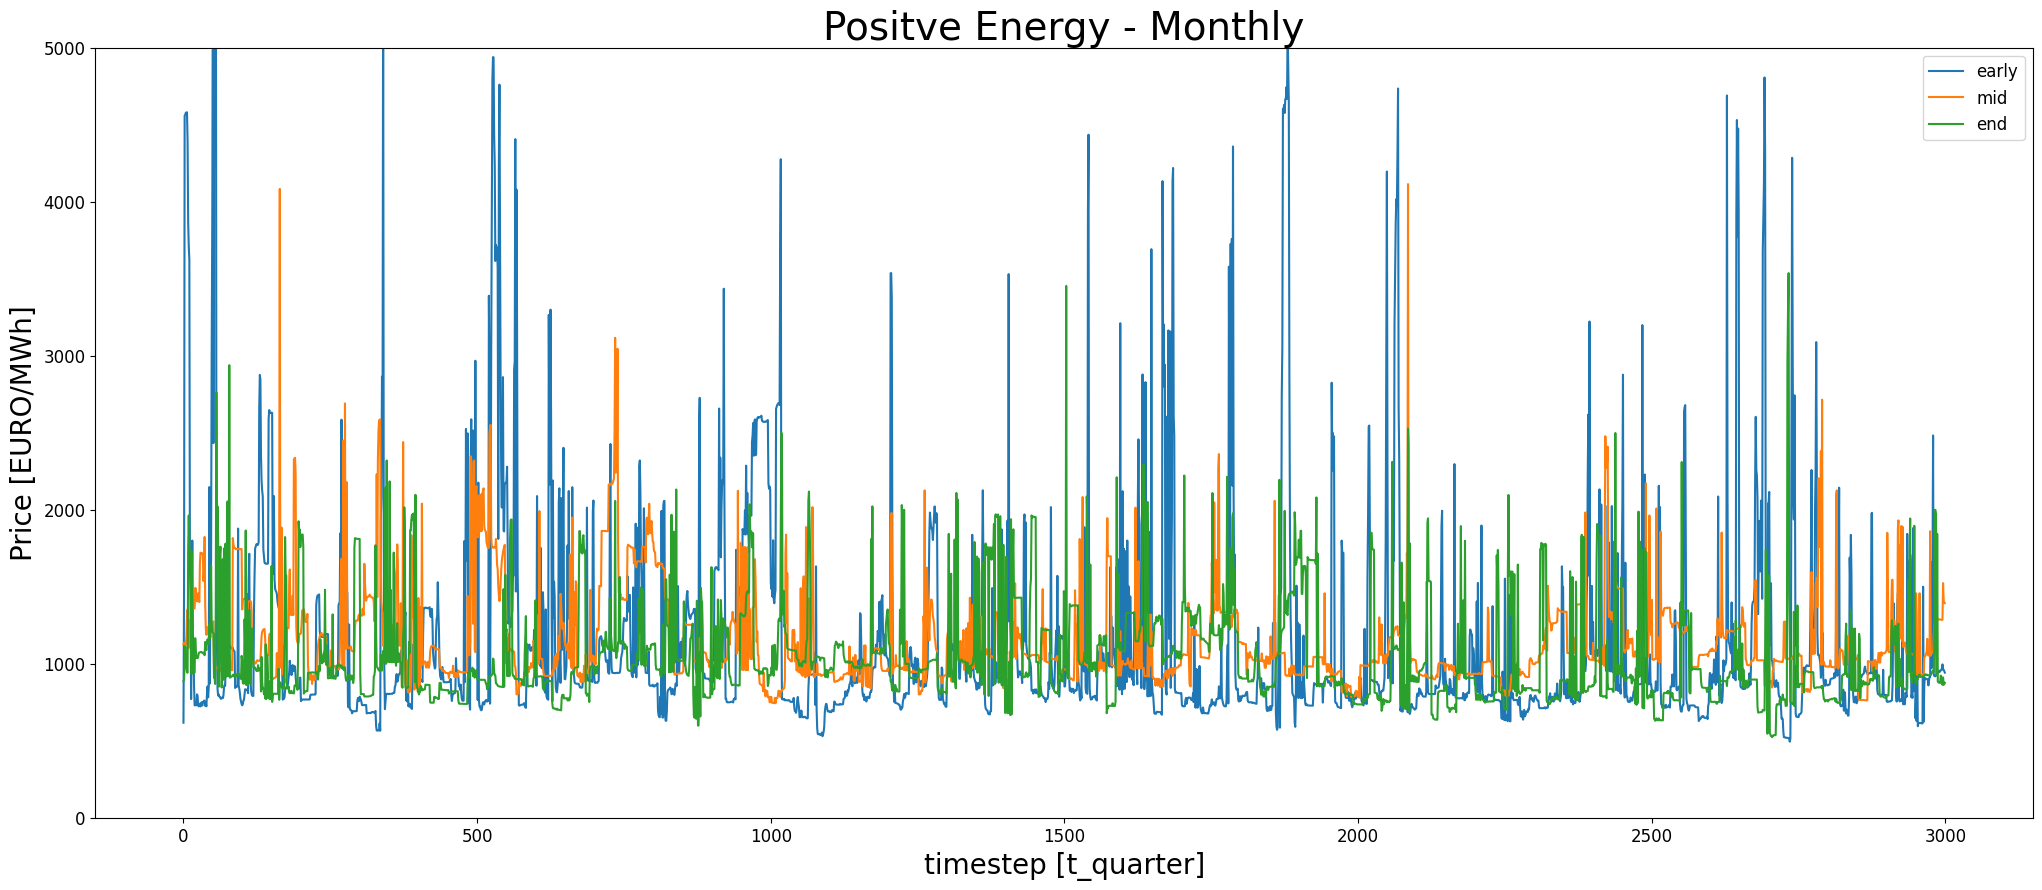
\includegraphics[width=1\linewidth]{pictures/posEngOverview.png}
	\caption{Overview Positive Energy Price}
	\label{fig:posEngOverview}
\end{figure}
\todo{das ist eine grafik mit den alten average preise, mache eine graifk mit den richtigen grenzpreisen}
\todo{grafiken verschiedene Preisszenarien}
\todo{appendix verweis zu python code}

Since no reliable forecasts can be made, real-world data is used for scenario generation.
For this purpose, data from the year 2023 was employed [see Table \ref{tab:energy_sources_std}].
It is observed that solar and onshore wind power plants are particularly subject to volatile production patterns.

\begin{table}[ht]
	\centering
	\begin{tabular}{|l|r|}
		\hline
		\textbf{Source}                 & \textbf{Standard Deviation} \\
		\hline
		Geothermal                      & 5.956190                    \\
		Fossil Oil                      & 85.360298                   \\
		Waste                           & 133.320136                  \\
		Hydro Water Reservoir           & 167.126363                  \\
		Hydro Run-of-river and poundage & 310.405850                  \\
		Biomass                         & 429.594441                  \\
		Nuclear                         & 1223.169733                 \\
		Hydro Pumped Storage            & 1543.402759                 \\
		Wind Offshore                   & 1833.588012                 \\
		Fossil Gas                      & 2916.794393                 \\
		Fossil Hard coal                & 3364.505964                 \\
		Fossil Brown coal/Lignite       & 3799.694920                 \\
		\textbf{Solar}                  & \textbf{9879.907341}        \\
		\textbf{Wind Onshore}           & \textbf{10506.831136}       \\
		\hline
	\end{tabular}
	\caption{Standard deviation per energy generator type}
	\label{tab:energy_sources_std}
\end{table}

Subsequently, the total production from solar and onshore wind is calculated for each time point,
and divided by the total production of all power plants at the same time.
This provides the relative share of these particularly volatile power plants in the overall production.
The relative hourly production is then used to determine daily average values.

The hypothesis is that if a prediction error occurs, it has a particularly strong impact when it occurs on days
with a high share of volatile production in the overall output.

These relative production data of volatile power plants are then divided into 36 quantiles.
The first, median, and last quantiles are used for scenario generation.

For this, the time points of the quantiles, now based on daily data, are extrapolated to a quarter-hourly rhythm,
and the corresponding market data from the other markets for the respective time periods are exported.
Simultaneously, the matching time periods from the DA and aFFR time series are also exported.

This results in 10 possible scenarios for days with high, medium, and low shares of volatile production.
The probabilities are assumed to be evenly distributed, thus each scenario-day has a probability of 10\%.




\todo{Python Code appendix verweis}


%--> kann über  mondpreis eskapen\\
%--> können eine kaum genutzte szenarioeplosion vermeiden (wording nochmal überarbeiten)\\
%- vereinfachung der RL markt mechanik/restriktionen
%--> stellen über batterie gleichung sicher das wir immer liefer können und vermeiden so komplexe $q_RA$ restriktionen (wann wie wo gelten)\\
%--> wir stellen einfach sicher das wir immer liefern könnten und fertig\\


- verschiedene Methoden ...\\
-> implementiert in python\\
-> alle können dem model hinzugefügt werden\\
-> ich habe dann aus diesen und jenen gründe diese Variante gewählt\\
